\subsection{System Testing}\label{subsec:systemtesting}
An important factor to validate is the impact on trip-scores caused by the diversity of users' smartphones. In a usage based insurance context, users needs to be treated equally, which relies entirely upon their smartphone and the GPS device inside. E.g. two smartphones logging the same trip, should report the same tripscore. Such an analysis can be quite extensive, involving an entire market of smartphones and different versions of GPS devices. Instead, a small applicability test will tell whether this system is vulnerable to GPS inaccuracy. 

An applicability test was conducted by bringing five different smartphones and two high quality GPS trackers into the same car, and recording the trip with all entities at the same time. If the system is applicable for usage based insurance, the smartphones needs to report the same tripscores, and the route needs to be highly similar to those recorded by the high quality GPS trackers. 

With these seven devices, four trips were completed driving around in northern Jutland, in the area of Aalborg. Raw data from the trips can be seen in appendix \ref{app:rawtestdata}. A summary of the tripscores for each phone, during the four trips, can be seen in table \ref{tab:smartphone_test}.

\begin{table*}[tb]
\centering
\caption{The tripscores from all seven recording devices, on all four trips used in the test, can be seen in this table}
\label{tab:smartphone_test}
\begin{tabular}{lllllllll}
       & Trip length & OnePlus One & Samsung G. S5 & HTC One Mini 2 & Huawei Y330 & Samsung G. S4 & BT-Q1300ST(\#1) & BT-Q1300ST(\#2) \\
Trip 1 & ~36200 & 50190.9     & 40091.5       & 75063.2        & 81819.4 & 37010.3       & 37909.8         & 69955.7         \\
Trip 2 & ~28200 & 58922.3     & 56780.8       & 28734.2        & 128056  & 27761.6       & 25372.5         & 72784.6         \\
Trip 3 & ~13400 & 42751.4     & 24026         & 21012.4        & 50622.1 & 16927.1       & 20980.8         & 85138.6         \\
Trip 4 & ~14400 & 23228.1     & 27530.3       & 19202.5        & 13082.1 & 18824.8       & 23916.6         & 27074.8        
\end{tabular}
\end{table*}

When examining trip 1 from table \ref{tab:smartphone_test} which has a length of approximately 36200 meters, two smartphones and one high quality GPS gets a score ranging from 37000-40000 which is good. But the remaining four tripscores disagree with varying severity. The worth is the Huawei Y330, which score this trip 81819.4. However, the Huawei Y330 only logs 23\% of the average GPS-coordinates compared to the other devices. The Huawei continues this trend throughout the test, and seems unfit for use in usage based insurance. Another alarming result is the degree to which the two high quality GPS devices disagrees. One scores the trip 37909.8 and the other 69955.7 which is a big difference.

Looking at trip 2 from table \ref{tab:smartphone_test} which has a length of approximately 28200 meters, three devices range from 25000-28750 in tripscore. The noteworthy result compared to trip 1 is, that the three devices with a low tripscore are not the same as those in trip 1.

The same pattern reoccur with trip 3 from table \ref{tab:smartphone_test}, which has a length of approximately 13400, but this time four devices gets a score ranging from 16500-24050, which are rather similar. The last three devices got a much higher tripscore, the highest being 85138.6, approximately 535\% above the trip-length, and it was logged by one of the high quality GPS devices. To highlight the disagreement between the two high quality GPS devices, the other device got a score of 20980.8. 

The pattern is broken with trip 4 from table \ref{tab:smartphone_test}, where all devices range between 13000-27550. This may still be somewhat diversified scores, but to compare it to trip 3, the highest device only scored approximately 91\% above the trip-length from this trip. The two high quality GPS devices also fairly agrees on the tripscore for trip 4, 23916.6 and 27074.8 respectively. 

When analyzing the results from this test, the immediate thought may be to throw away the smartphone as usage based insurance component. The concern about accuracy, integrity, availability and continuity of service in stand-alone GPS receivers is also raised in\citep{art:challenges_smartphone_ubi} \citep{art:survey_mobile_phone_sensing} \citep{art:smartphones_for_monitoring_and_ubi} \citep{art:insurtelematics} \citep{art:in-car_positioning_technologies}. But two other factors may have influenced the results in table \ref{tab:smartphone_test}. The first factor is GPS interference, in which case the test-setup could have changed the results we received, because all the GPS devices was kept close together in a fabric container and placed in the front of the car near the windshield. This could affect the GPS receivers in each device by them interfering with each other\citep{art:gps_interference_one} \citep{art:gps_interference_two}. This position was decided upon, because a common reference point was valued in the applicability test. 

The second factor is the use of third party software for map-matching of the spatio-temporal trajectories collected by the smartphones, called TrackMatching\citep{trackmatch}. TrackMatch attempts to mapmatch a series of spatio-temporal points to the OSM road network, and output the entire route by segments and map-adjusted GPS points. How TrackMatch decides to readjust these GPS points are outside our control, and we did not implement a module to oversee this readjusting, so this influence cannot be changed. 

It was decided to repeat the applicability test and eliminate the GPS interference as much as possible. This was done by spreading each GPS device out inside the car, and create as much space between them as possible. The possible margin of error by using a separated reference point was disregarded. 

TABEL WITH NEW TEST DATA???

The test shows once again a considerable difference, when we compare the two high quality GPS devices. But the difference is decreased substantially compared to the first test, which signifies that some external influence may have been affecting the devices. Looking at the raw data in \textbf{appendix X og Y},an observation is that their behavior is consistent. When looking at the amount of accelerations, brakes and jerks they count, one device consistently counts more than the other. 7777 counted a total of 1529 of these events, whereas 888 8 counted a total of 3894, which is 191.125 events per trip on average for 7777, and 486.75 events per trip on average for 8888. This signifies that it may not be able to conclude any comparison between these two, because they deliver such different results.









[6] F. Calabrese, M. Colonna, P. Lovisolo, D. Parata, and C. Ratti, “Realtime urban monitoring using cell phones: A case study in Rome,” IEEE Trans. Intell. Transp. Syst., vol. 12, pp. 141–151, Mar. 2011.
-Furthermore, as a result of signal multipath and urban canyon obstructions, GPSs do not work well in urban areas.
-Finally, privacy legislation requires careful contractual work, as vehicle owners must explicitly agree to share their location for the purpose of automobile traffic estimation.
-More focused on traffic monitoring - we focus on fine-grained gps results to verify driver profiles

[7]N. Lane, E. Miluzzo, H. Lu, D. Peebles, T. Choudhury, and A. Campbell, “A survey of mobile phone sensing,” IEEE Commun. Mag., vol. 48, pp. 140–150, Sept. 2010.
-technical barrier related to performing privacy-sensitive and resource-sensitive reasoning with noisy data and noisy labels, and providing useful effective feedback to user.


[10] P. Händel, J. Ohlsson, M. Ohlsson, I. Skog, and E. Nygren, “Smartphone-based measurement systems for road vehicle traffic monitoring and usage-based insurance,” IEEE Syst. J., vol. PP, pp. 1–11, Mar. 2014
-Primary goal is to monitor traffic, secondary to generate revenue through UBI and based on driver profiles
-[10]-[12]
-speeding, cornering, braking, and accelerating habits; the time and date; and the road conditions.
-In this paper, findings are presented from the first ever trial of a smartphone-based UBI, where the smartphone is used as an advanced measurement probe in a complex measurement system.
-Road vehicle positioning and navigation technologies based on stand-alone GPS receivers are vulnerable because of the low signal levels and requirement of line of sight and, thus, have to be supported by additional information sources to obtain the desired accuracy, integrity, availability, and continuity of service [33], [34].
-mathematical models of vehicle motion [33], [34].
-sensor fusion for better results


Insurance Telematics: Opportunities and Challenges with the Smartphone Solution
-The data quality provided by the smartphone is characterized in terms of Accuracy, Integrity, Availability, and Continuity of Service.
-revealing the obstacles that have to be combated for a successful smartphone-based installation, which are the poor integrity and low availability.
-The satellite based positioning reported a coverage in the interval 60 \% to 99.7 \%, for the individual smartphones.

[27]I. Skog, P. Händel, M. Ohlsson, and J. Ohlsson, “Challenges in smartphone-driven usage based insurance,” in Proc. IEEE Global Conf. Signal Information Processing, Austin, TX, Dec. 2013.
-Insurance telematics employ parameters to evaluate the risk associated with a driver of a car, like time of the day, location or road taken, distance traveled, and driving behavior characteristics like heavy breaking, acceleration, cornering, swerving, smoothness and speeding.
-Dicussing the challenges with using the semi unreliable smartphone GPS. Suggests model based signal processing, taking in non-equidistant sampling into account, in combination with tailored outlier rejection scheme.


[33] I. Skog and P. Händel, “In-car positioning and navigation technologies— A survey,” IEEE Trans. Intell. Transp. Syst., vol. 10, no. 1, pp. 4–21, Mar. 2009.
-Focus more of in-car navigation systems than GPS in smartphones.
-Positioning technologies based on stand-alone GPS receivers are vulnerable and, thus, have to be supported by additional information sources to obtain the desired accuracy, integrity, availability, and continuity of service.

beskriv resultaterne, måske overordnet, med rå-data i appendix.

There are a couple of issues regarding this applicability test. 
GPS interference
\subsection{Pearson Correlation}\label{subsec:pearsoncorrelation}

In order to test the validity of our metrics and the chosen policy, a the pearson correlation between the metrics have been conducted. The point of the test is to make sure no metrics are directly correlating, meaning one of the metrics is negligible. There is a number of different reasons as to why the outcome will look as it does, and it will be discussed thoroughly. The Pearson-Correlation have been calculated on the individual scores given to a trip per each of metrics. 

The matrix of pearson correlations between the metrics is shown at table \ref{tab:pearsonmatrix}. The most notable result is the multicollinearity between accelerations and brakes, which seems rather odd as they are diametrical opposites and can per definition not exist at the same time. Another highly correlating metric is jerks having a correlation of 0.828 with both brakes and accelerations. 

\begin{table*}[tb]
\centering
\caption{This is the pearson correlation matrix between the metrics}
\label{tab:pearsonmatrix}
\begin{tabular}{l|llllll}
                      & Roadtypes & Critical Time Periods & Speeding & Accelerations & Brakes & Jerks  \\ \hline
Roadtypes             & 1         & -0.250                & -0,546   & -0.341        & -0,348 & -0,241 \\
Critical Time Periods & -0.250    & 1                     & 0.156    & 0.460         & 0.428  & 0.313  \\
Speeding              & -0,546    & 0.156                 & 1        & 0.196         & 0.195  & 0.144  \\
Accelerations         & -0.341    & 0.460                 & 0.196    & 1             & 0.971  & 0.828  \\
Brakes                & -0,348    & 0.428                 & 0.195    & 0.971         & 1      & 0.828  \\
Jerks                 & -0,241    & 0.313                 & 0.144    & 0.828         & 0.828  & 1     
\end{tabular}
\end{table*}

Looking closer at the multicollinearity between accelerations and brakes, there is a couple of different factors which affect the result. As mentioned accelerating and braking are diametrically opposite, but they are both dependant of the speed of the vehicle (as they are calculated through the change in speed). If the driver performs a big acceleration, his speed is high and he at some point needs to brake in order to decline in speed. 

\begin{figure}[tb]
\centering
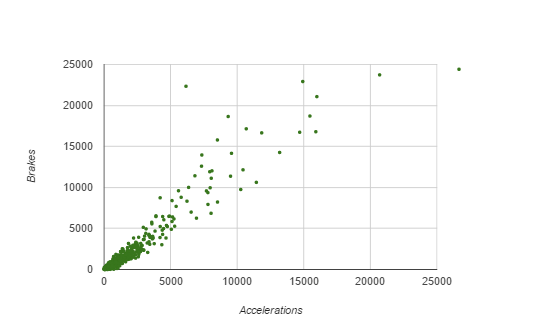
\includegraphics[width=0.465\textwidth]{Pictures/abcorrel}
\caption{The correlation between accelerations and brakes}
\label{fig:abcorrel}
\end{figure}

The figure shown at \ref{fig:abcorrel} clearly illustrates the correlation. Another reasoning as to why these metrics correlate can be the thresholds in the policy used to calculate the scores. As earlier mentioned the threshold for brakes are 8 $m/s^2$ whereas accelerations are counted from 5 $m/s^2$. If we had no thresholds and the delinquencies were scored the same, the correlation would be 1.0 as it only depended on the speed of the vehicle. 
Jerks was the metric met with the highest level of scepticism when implemented, and the correlation shows that it was not completely unwarranted. It does show a lot of correlation with both brakes and accelerations. The figure \ref{fig:ajcorrel} shows the correlation between accelerations and jerks. Jerks are as mentioned calculated as $m/s^3$, and a driver with many accelerations are almost bound to have a lot of jerks as it is hard to keep a constant acceleration.

\begin{figure}[tb]
\centering
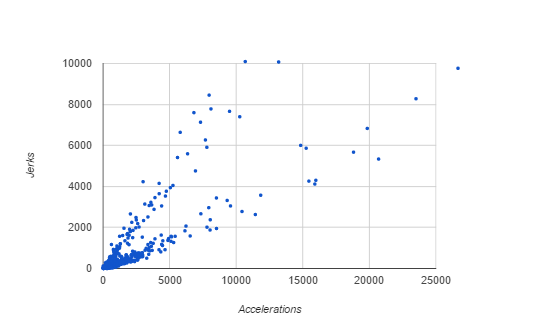
\includegraphics[width=0.465\textwidth]{Pictures/ajcorrel}
\caption{The correlation between accelerations and jerks}
\label{fig:ajcorrel}
\end{figure}


the similar correlation between the two can be answered by the correlation between accelerations and brakes. 

